\documentclass[12pt]{article}
\usepackage[left=1cm, right=1cm, top=2cm,bottom=1.5cm]{geometry} 

\usepackage[parfill]{parskip}
\usepackage[utf8]{inputenc}
\usepackage[T2A]{fontenc}
\usepackage[russian]{babel}
\usepackage{enumitem}
\usepackage[normalem]{ulem}
\usepackage{amsfonts, amsmath, amsthm, amssymb, mathtools}
\usepackage{tabularx}
\usepackage{hhline}

\usepackage{accents}
\usepackage{fancyhdr}
\pagestyle{fancy}
\renewcommand{\headrulewidth}{1.5pt}
\renewcommand{\footrulewidth}{1pt}

\usepackage{graphicx}
\usepackage[figurename=Рис.]{caption}
\usepackage{subcaption}
\usepackage{float}

%%Наименование папки откуда забирать изображения
\graphicspath{ {./images/} }

%%Изменение формата для ввода доказательства
\renewcommand{\proofname}{$\square$  \nopunct}
\renewcommand\qedsymbol{$\blacksquare$}

%%Изменение отступа на таблицах
\addto\captionsrussian{%
	\renewcommand{\proofname}{$\square$ \nopunct}%
}
%% Римские цифры
\newcommand{\RN}[1]{%
	\textup{\uppercase\expandafter{\romannumeral#1}}%
}

%% Для удобства записи
\newcommand{\MR}{\mathbb{R}}
\newcommand{\MQ}{\mathbb{Q}}
\newcommand{\MN}{\mathbb{N}}
\newcommand{\MI}{\mathrm{I}}
\newcommand{\MJ}{\mathrm{J}}
\newcommand{\MH}{\mathrm{H}}
\newcommand{\MT}{\mathrm{T}}
\newcommand{\MU}{\mathcal{U}}
\newcommand{\MV}{\mathcal{V}}
\newcommand{\VN}{\varnothing}
\newcommand{\VE}{\varepsilon}

\theoremstyle{definition}
\newtheorem{defn}{Опр:}
\newtheorem{rem}{Rm:}
\newtheorem{prop}{Утв.}
\newtheorem{exrc}{Упр.}
\newtheorem{lemma}{Лемма}
\newtheorem{theorem}{Теорема}
\newtheorem{corollary}{Следствие}

\newenvironment{cusdefn}[1]
{\renewcommand\thedefn{#1}\defn}
{\enddefn}

\DeclareRobustCommand{\divby}{%
	\mathrel{\text{\vbox{\baselineskip.65ex\lineskiplimit0pt\hbox{.}\hbox{.}\hbox{.}}}}%
}
%Короткий минус
\DeclareMathSymbol{\SMN}{\mathbin}{AMSa}{"39}
%Длинная шапка
\newcommand{\overbar}[1]{\mkern 1.5mu\overline{\mkern-1.5mu#1\mkern-1.5mu}\mkern 1.5mu}
%Функция знака
\DeclareMathOperator{\sgn}{sgn}

%Обозначение константы
\DeclareMathOperator{\const}{\text{const}}

%Интеграл в большом формате
\DeclareMathOperator{\dint}{\displaystyle\int}

\newcommand{\smallerrel}[1]{\mathrel{\mathpalette\smallerrelaux{#1}}}
\newcommand{\smallerrelaux}[2]{\raisebox{.1ex}{\scalebox{.75}{$#1#2$}}}

\newcommand{\smallin}{\smallerrel{\in}}
\newcommand{\smallnotin}{\smallerrel{\notin}}

\newcommand*{\medcap}{\mathbin{\scalebox{1.25}{\ensuremath{\cap}}}}%
\newcommand*{\medcup}{\mathbin{\scalebox{1.25}{\ensuremath{\cup}}}}%

%Скалярное произведение
\DeclarePairedDelimiterX{\inner}[2]{\langle}{\rangle}{#1, #2}

%Подпись символов снизу
\newcommand{\ubar}[1]{\underaccent{\bar}{#1}}

\begin{document}
\lhead{Математический анализ - \RN{2}}
\chead{Шапошников С.В.}
\rhead{Лекция - 12}
	
\section*{Линейные функции}
Пусть $X$ и $Y$ - нормированные пространства. $L \colon X \to Y$ - линейное отображение.
\begin{defn}
	Отображение $L \colon X \to Y$ называется \uwave{линейным} (или еще говорят линейным оператором), если выполнено следующее равенство: 
	$$
		L(\alpha_1 x + \alpha_2 y) = \alpha_1 L(x) + \alpha_2 L(y), \, \forall \alpha, \beta \in \MR, \, x,y \in X
	$$ 
\end{defn}

\subsection*{Непрерывность линейных отображений}
\textbf{\uline{Конечномерный случай}}: Линейные отображения $L \colon \MR^n \to \MR^m$ задаются следующим образом:
$$
	L(x) = \underset{m \times n}{A}x
$$
У этого отображения $k$-ый столбец матрицы $A$ равен $L(e_k)$, где $e_k = \begin{pmatrix} 0 &	\dotsc & 0 & 1 & 0 & \dotsc & 0 \end{pmatrix}^T$. В частном случае $m = 1$ это видно сразу, поскольку оператор будет иметь следующий вид 
$$
	L(x) = a_1 x_1 + \dotsc + a_n x_n 
$$ 
Если координаты к чему-то стремятся, то это выражение будет стремится к сумме произведения коэффициентов на координатные пределы. Следовательно, в конечномерных случаях имеем непрерывные функции, как комбинацию непрерывных функций.

\textbf{\uline{Бесконечномерный случай}}:  В этом случае непрерывности может не быть: 
$$
	L\colon C^1[0,1] \to \MR,\, L(f) = f^\prime(0)
$$
$L$ - не является непрерывным отображением, но это линейное отображение.

\begin{theorem}
	Пусть $X$ и $Y$ - нормированные пространства. $L\colon X \to Y$ - линейная функция, тогда следующие утверждения равносильны:
	\begin{enumerate}[label ={(\arabic*)}]
		\item $L$ - непрерывна;
		\item $L$ - непрерывна в $0$;
		\item $\exists \, C > 0 \colon \|L(x)\|_Y \leq C \|x\|_X, \, \forall x$;
	\end{enumerate}
\end{theorem}
\begin{proof}\hfill\\
	$(1) \Rightarrow (2)$ Очевидно: если функция непрерывна, то она непрерывна в $0$.
	
	$(2) \Rightarrow (3)$ Функция $L$ непрерывна в $0 \Rightarrow$ ограничена в окрестности $0$, тогда: 
	$$
		\exists \, C_1 > 0, \, \exists \, B(0,\delta) \colon \|L(x)\| \leq C_1, \, \forall x \in B(0,\delta)
	$$
	Пусть $x \neq 0 \Rightarrow$ рассмотрим вместо $x$ следующий вектор: $\dfrac{\delta}{2}{\cdot}\dfrac{x}{\|x\|}$, длина этого вектора равна $\dfrac{\delta}{2}$. Тогда: 
	$$
		\dfrac{\delta}{2}{\cdot}\dfrac{x}{\|x\|} \in B(0, \delta) \Rightarrow \bigg\|L\bigg(\dfrac{\delta}{2}{\cdot}\dfrac{x}{\|x\|} \bigg) \bigg\| = 
		\bigg\|\dfrac{\delta}{2}{\cdot}\dfrac{1}{\|x\|} L(x) \bigg\| = \dfrac{\delta}{2}{\cdot}\dfrac{1}{\|x\|}{\cdot} \|L(x) \| \leq C_1 \Rightarrow \|L(x)\| \leq \dfrac{2C_1}{\delta}\|x\| = C \|x\| 
	$$
	
	$(3) \Rightarrow (1)$ $\|L(x-y)\| = \|L(x) - L(y)\| \leq C\|x - y\| \Rightarrow$ по определению непрерывности $L$ - непрерывна.
\end{proof}

\subsection*{Линейное пространство линейных непрерывных операторов}
$\mathcal{L}(X,Y)$ - линейное пространство линейных непрерывных (ограниченных) операторов (функций, отображений). Пусть $L \in \mathcal{L}(X,Y)$, определим норму 
$$
	\|L\| = \sup\limits_{x \neq 0} \dfrac{\|L(x)\|}{\|x\|}
$$
Данный супремум конечен из-за свойства $(3)$ теоремы выше.

\begin{exrc}
	Проверить, что пространство $\mathcal{L}$ с указанной выше нормой: $(\mathcal{L}, \| \cdot \|)$ - нормированное.
\end{exrc}
\begin{proof}
	Поскольку пространство линейное, то нам необходимо проверить свойства нормы:
	\begin{enumerate}[label ={(\arabic*)}]
		\setcounter{enumi}{-1}
		\item Выполнено по определению функции $\|\cdot\|_X$, так как $x \neq 0 \Rightarrow \|x\|_X > 0 \Rightarrow \sup\limits_{x \neq 0} \dfrac{\|L(x)\|_Y}{\|x\|_X} \geq 0$;
		
		\item $\|L\| = 0 \Leftrightarrow \forall x \neq 0, \, \|L(x)\|_Y = 0 \Leftrightarrow  \forall x \neq 0, \, L(x) = 0$, а поскольку $L(0) = L(0) + L(0) \Rightarrow L(0) = 0$, то получим, что $L(x) = 0, \, \forall x \in X \Leftrightarrow L = 0$;
		
		\item $\|\alpha L\| = \sup\limits_{x \neq 0} \dfrac{\|\alpha L(x)\|}{\|x\|} = \sup\limits_{x \neq 0} \dfrac{|\alpha|{\cdot}\| L(x)\|}{\|x\|} = |\alpha|{\cdot}\sup\limits_{x \neq 0} \dfrac{\|L(x)\|}{\|x\|} = |\alpha|{\cdot}\|L\|, \, \forall \alpha \in \MR$;
		\item $\dfrac{\|L(x) + M(x)\|}{\|x\|} \leq \dfrac{\|L(x)\|}{\|x\|} + \dfrac{\| M(x)\|}{\|x\|} \leq \|L\| + \|M\| \Rightarrow \|L + M\| = \sup\limits_{x \neq 0} \dfrac{\|L(x) + M(x)\|}{\|x\|} \leq \|L\| + \|M\|$;
	\end{enumerate}
	Таким образом, все свойства нормы выполнены и пространство является нормированным.
\end{proof}
\begin{rem}
	Сделаем ряд замечаний, относительно конечномерных случаев:
	\begin{enumerate}[label ={\arabic*)}]
		\item 	Пусть $L \colon \MR^n \to \MR$, тогда $L(x) = a_1 x_1 + \dotsc + a_n x_n = \langle a,x \rangle \Rightarrow \|L(x) \| = |L(x)|$, поскольку находимся в простренстве $\MR$. Тогда, в силу неравенства Коши-Буняковского $|L(x)| \leq \|a\|{\cdot}\|x\|$. Отсюда следует, что $L$ - непрерывное линейное отображение;
		\item Пусть $L \colon \MR^n \to \MR^m$, тогда 
		$
			L(x) = 
			\begin{pmatrix}
				L_1(x)\\
				L_2(x)\\
				\vdots\\
				L_m(x)
			\end{pmatrix}
		$ - координаты вектора, который получается отображением $x \in \MR^n$. Очевидно, что $L_k \colon \MR^n \to \MR$ - линейно (следует из покоординатного сложения) 
		$$
			L(\alpha x + \beta y) = 
			\begin{pmatrix}
				L_1(\alpha x + \beta y)\\
				L_2(\alpha x + \beta y)\\
				\vdots\\
				L_m(\alpha x + \beta y)
			\end{pmatrix}
			= \alpha L(x) + \beta L(y) = \alpha
						\begin{pmatrix}
				L_1(x)\\
				L_2(x)\\
				\vdots\\
				L_m(x)
			\end{pmatrix} + \beta 
			\begin{pmatrix}
				L_1(y)\\
				L_2(y)\\
				\vdots\\
				L_m(y)
			\end{pmatrix}
		$$
		тогда, в силу первого пункта замечания: 
		$$
			|L_k(x)| \leq C_k\|x\|
		$$ 
		Отсюда мы получаем следующее: 
		$$
			\|L(x)\| \leq \|C\|{\cdot}\|x\| = \sqrt{\displaystyle\sum\limits_{k}C_k^2}{\cdot} \|x\|
		$$
		Таким образом, $L$ - непрерывный линейный оператор. 
	\end{enumerate}
\end{rem}

\newpage
\section*{Дифференцируемые отображения}
Пусть $X$ и $Y$ - нормированные пространства и $a \in X$. Предположим, что $f \colon U \to Y$, где $U$ - открытое множество, содержащее $a$, то есть $f$ определена в окрестности точки $a$.

\begin{defn}
	Функция $f$ \uwave{дифференцируема} в точке $a$, если существует непрерывное линейное отображение $L\colon X \to Y$ и функция $\alpha \colon X \to Y$ такие, что:
	$$
		f(a + h) - f(a) = L(h) + \alpha(h){\cdot}\|h\|, \, \alpha(h) \colon \lim\limits_{h \to 0}{\alpha(h)} = 0
	$$ 
\end{defn}
\textbf{Пример}: Пусть $L \colon X \to Y$ - линейная непрерывная функция, тогда $L$ - дифференцируема в каждой точке. Действительно:
$$
	L(a+h) - L(a) = L(a + h - a) =  L(h) + 0{\cdot}\|h\|
$$
\begin{prop}
	Если $f$ дифференцируема в точке $a$, то $f$ непрерывна в точке $a$.
\end{prop}
\begin{proof}
	$f(a+h) - f(a) = L(h)  + \alpha(h){\cdot}\|h\| \xrightarrow[h\to 0]{} L(0) + 0 = 0 \Rightarrow \lim\limits_{x \to a}f(x) = f(a)$, поскольку $L(h)$ - непрерывная линейная функция и $x = a + h,\, h \to 0 \Leftrightarrow x \to a$.
\end{proof}
\begin{rem}
	Дифференцируемые функции всегда непрерывны, поэтому в качестве недифференцируемых функций подойдут линейные разрывные.
\end{rem}
\begin{theorem}
	$f$ дифференцируема в точке $a \Leftrightarrow$ существует линейное непрерывное отображение $L$ такое, что:
	$$
		\lim\limits_{h \to 0} \dfrac{\|f(a+h) - f(a) - L(h)\|}{\|h\|} = 0
	$$
	В частности, если $f$ дифференцируема в точке $a$ и $L$ - линейная часть приращения $f$, то: 
	$$
		\forall v, \, \lim\limits_{t \to 0} \dfrac{f(a + tv) - f(a)}{t} = L(v)
	$$
\end{theorem}
\begin{rem}
	В прошлом семестре, дифференцируемость давалась через: $f(a+h) - f(a) = Ah + \alpha(h){\cdot}h$. После чего, давалось определение производной: $f^\prime(a) = \lim\limits_{h \to 0}\dfrac{f(a+h) - f(a)}{h}$. Затем давалось, что дифференцируемость и существование производной равносильны и если $f$ - дифференцируема, то $A = f^\prime(a)$.
\end{rem}
\begin{rem}
	Если не брать предел по $h$, который подходит произвольно к нулю, а брать как предел подходящий к нулю вдоль вектора $v$, то получим ситуацию аналогичную одномерному случаю.
\end{rem}
\begin{proof}
	Функция $f$ - дифференцируема в точке $a \Leftrightarrow f(a+h) - f(a) = L(h) + \alpha(h){\cdot}\|h\|, \, \lim\limits_{h \to 0}{\alpha(h)} = 0$, но это то же самое, что:
	$$
		\dfrac{f(a+h) - f(a) - L(h)}{\|h\|} = \alpha(h) \to 0 \Leftrightarrow \lim\limits_{h \to 0} \|\alpha(h) \| = 0 \Leftrightarrow \lim\limits_{h \to 0} \dfrac{\|f(a+h) - f(a) - L(h)\|}{\|h\|} = 0
	$$
	Рассмотрим частный случай и возьмем $h = tv, \, v \neq 0$, тогда:
	$$
		\dfrac{f(a + tv) - f(a) - L(tv)}{\|tv\|} \xrightarrow[t \to 0]{} 0 \Leftrightarrow \dfrac{1}{\|v\|}{\cdot}\dfrac{t}{|t|}{\cdot}\bigg(\dfrac{f(a + tv) - f(a)}{t} - L(v)\bigg) \xrightarrow[t \to 0]{} 0
	$$
	Поскольку $\bigg\|\dfrac{1}{\|v\|}{\cdot}\dfrac{t}{|t|}\bigg\| = \bigg|\dfrac{1}{\|v\|}{\cdot}\dfrac{t}{|t|}\bigg| = \dfrac{1}{\|v\|} \neq 0$, то получаем, что: 
	$$
		\lim\limits_{t \to 0} \dfrac{f(a + tv) - f(a)}{t} - L(v) = 0 \Rightarrow 
		 \lim\limits_{t \to 0} \dfrac{f(a + tv) - f(a)}{t} = L(v)
	$$
\end{proof}
\begin{defn}
	Предел $\lim\limits_{t \to 0} \dfrac{f(a + tv) - f(a)}{t}$ называют \uwave{производной функции} $f$ \uwave{по вектору} $v$ и обозначают следующим образом: 
	$$
		\dfrac{\partial f}{\partial v}(a) = \lim\limits_{t \to 0} \dfrac{f(a + tv) - f(a)}{t}
	$$
\end{defn}
\begin{rem}
	Если $\|v\| = 1$, то эту производную $\dfrac{\partial f}{\partial v}(a)$ еще называют \uwave{производной по направлению}. Иногда требуют, чтобы $t \to 0+$.
\end{rem}
\begin{corollary}
	$L(v) = \dfrac{\partial f}{\partial v}(a), \, \forall v$ и $L$ определено однозначно.
\end{corollary}
\begin{proof}
	Следует из доказательства для частного случая теоремы выше, поскольку значение этого отображения на векторе $v$ однозначно определено функцией $f$.
\end{proof}

\begin{defn}
	Линейный оператор $L$ из определения дифференцируемости $f$ называется \uwave{дифференциалом} $f$. Обозначается, как $df(a,h)$ или $df(h)$, если понимаем в какой точке все происходит.
\end{defn}

Тогда определение дифференцируемости записывается следующим образом:
\begin{defn}
	Функция $f$ \uwave{дифференцируема} в точке $a$, если выполнено следующее равенство:
	$$
		f(a + h) - f(a) = df(a,h) + \alpha(h){\cdot}\|h\|, \, \lim\limits_{h \to 0}{\alpha(h)} = 0
	$$
	где $h \mapsto df(a,h)$ - непрерывное линейное отображение, а также $df(a,v) = df(v) = \dfrac{\partial f}{\partial v}(a)$.
\end{defn}

\section*{Частные случаи дифференцируемости функций}
\subsection*{$(\RN{1})$ Отображения из $\MR^n$ в $\MR$}
Пусть $f \colon \MR^n \to \MR$ дифференцируема в точке $a = (a_1, \dotsc, a_n)$. Запишем определение дифференцируемости:
$$
	f(a_1 + h_1, \dotsc, a_n + h_n) - f(a_1, \dotsc, a_n) = df(\overrightarrow{h\,}) + \alpha(\overrightarrow{h\,}){\cdot}{\|\overrightarrow{h\,}\|}
$$
где $df(\overrightarrow{h\,})$ - линейное отображение из $\MR^n$ в $\MR$, тогда: 
$$
	df(h) = h_1 {\cdot} df(e_1) + \dotsc + h_n {\cdot} df(e_n), \, e_k = \begin{pmatrix} 0 &	\dotsc & 0 & 1 & 0 & \dotsc & 0 \end{pmatrix}^T
$$ 
По определению $df(e_k) = \dfrac{\partial f}{\partial e_k}(a) = \lim\limits_{t \to 0} \dfrac{f(a + te_k) - f(a)}{t}$, то есть фиксируем все координаты значениями $a_j$, кроме $k$-ой координаты:
$$
	\lim\limits_{t \to 0} \dfrac{f(a + te_k) - f(a)}{t} = \lim\limits_{t \to 0} \dfrac{f(a_1, \dotsc,a_{k-1}, a_k + t, a_{k+1}, \dotsc, a_n) - f(a_1, \dotsc,a_{k-1}, a_k, a_{k+1}, \dotsc, a_n)}{t}
$$
Таким образом, мы рассматриваем функцию $x_k \mapsto f(a_1,\dotsc, x_k,\dotsc, a_n)$ одной переменной $x_k$ и дифференцируем её по этой переменной.

\begin{defn}
	Производная вдоль вектора $e_k$: $\dfrac{\partial f}{\partial e_k}(a)$ называется \uwave{частной производной функции} $f$ \uwave{по переменной} $x_k$ \uwave{в точке $a$} и обозначается следующим образом: 
	$$
		\dfrac{\partial f}{\partial x_k}(a) = \dfrac{\partial f}{\partial e_k}(a) = \lim\limits_{t \to 0} \dfrac{f(a + te_k) - f(a)}{t}
	$$
\end{defn}

Частная производная означает дифференцирование вдоль координат. Таким образом, мы можем записать дифференциал в следующем виде:
$$
	df(h) =  \dfrac{\partial f}{\partial x_1}(a){\cdot}h_1 + \dotsc + \dfrac{\partial f}{\partial x_n}(a){\cdot} h_n
$$
\begin{defn}
	Вектор состоящий из частных производных $\Big(\dfrac{\partial f}{\partial x_1}(a), \dotsc, \dfrac{\partial f}{\partial x_n}(a)\Big)$ в точке $a$ называется \uwave{градиентом функции} $f$ и обозначается следующим образом: 
	$$
		\text{grad}\, f(a) = \nabla f(a) = \Big(\dfrac{\partial f}{\partial x_1}(a), \dotsc, \dfrac{\partial f}{\partial x_n}(a)\Big)
	$$
\end{defn}

Рассмотрим следующее выражение:
$$
	\dfrac{\partial f}{\partial v}(a) = \lim\limits_{t \to 0}\dfrac{f(a+tv) - f(a)}{t} = df(v) = \dfrac{\partial f}{\partial x_1}(a){\cdot}v_1 + \dotsc + \dfrac{\partial f}{\partial x_n}(a){\cdot} v_n = \inner{\nabla f(a)}{v}
$$
Таким образом, производная по направлению это скалярное произведение градиента с вектором $v$. Возникает вопрос, а что можно говорить о поведении функции, глядя на градиент?
\begin{figure}[H]
	\centering
	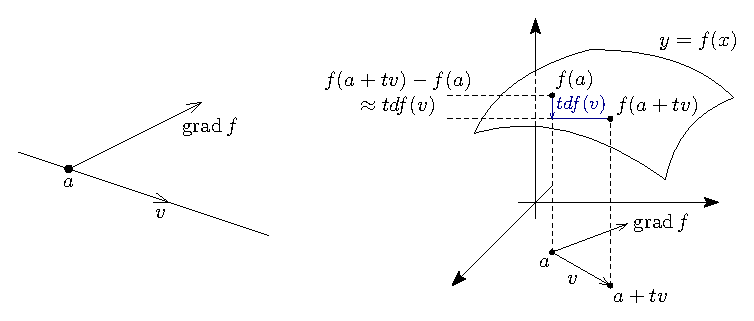
\includegraphics[width=0.85\textwidth]{12_1.eps}
	\caption{Геометрический смысл производной по вектору $v$.}
	\label{12_1}
\end{figure}
\uline{\textbf{Геометрический смысл производной по направлению}}: При достаточно маленьких значениях $t$, приращение функции $f$ в точке $a$ будет примерно равно $tdf(v) \approx f(a + tv) - f(a)$. Таким образом, производная по вектору $v$ указывает, как изменяется функция, когда мы сдвигаемся по вектору $v$. 

Но мы знаем, что $df(v) = \inner{\nabla f(a)}{v}$. Тогда если возьмем $v$ перпендикулярно градиенту, то скалярное произведение будет равно $0 \Rightarrow$ приращение функции примерно нулевое. То есть двигаясь вдоль градиента, значения функции остаются постоянными. Если будем двигаться в сторону градиента, то это скалярное произведение будет максимальным, в противоположную сторону - минимальным.

\begin{prop}
	Предположим, что $f \colon \MR^n \to \MR$ дифференцируема в точке $a$ и $\nabla f(a) \neq 0$. Тогда максимум производной функции $f$ по направлению $v$: $\max\limits_{\|v\| = 1}\dfrac{\partial f}{\partial v}(a)$ достигается на $v = \dfrac{\nabla f(a)}{\|\nabla f(a) \|}$ и соответственно минимум $\min\limits_{\|v\| = 1}\dfrac{\partial f}{\partial v}(a)$ достигается на $v = - \dfrac{\nabla f(a)}{\|\nabla f(a) \|}$.
\end{prop}
\begin{proof}
	Рассмотрим производную, как скалярное произведение: $ \dfrac{\partial f}{\partial v}(a) = \inner{\nabla f(a)}{v}$. Поскольку $\|v\| = 1$, используем неравенство Коши-Буняковского и получим следующий результат:
	$$
		- \|\nabla f(a)\|{\cdot}\|v\| = - \|\nabla f(a)\| \leq \dfrac{\partial f}{\partial v}(a) = \inner{\nabla f(a)}{v} \leq  \|\nabla f(a)\|{\cdot}\|v\| =  \|\nabla f(a)\| 
	$$
	Равенство возможно только тогда, когда $\nabla f(a)$ и $v$ - линейно зависимы, а поскольку $\|v\| = 1$, то для равенства в правой части $v = \dfrac{\nabla f(a)}{\|\nabla f(a) \|}$  и $v = -\dfrac{\nabla f(a)}{\|\nabla f(a) \|}$ для равенства в левой части.
\end{proof}

\textbf{Пример}: $f(x_1,x_2) = x_1^2 + x_2^2$, возьмем точку $(a_1,a_2)$ и найдем градиент функции в этой точке: 
$$
	\nabla f(a_1,a_2) = \Big(\dfrac{\partial f}{\partial x_1}(a_1,a_2), \dfrac{\partial f}{\partial x_2}(a_1,a_2)\Big) = (2a_1, 2a_2)
$$
\begin{figure}[H]
	\centering
	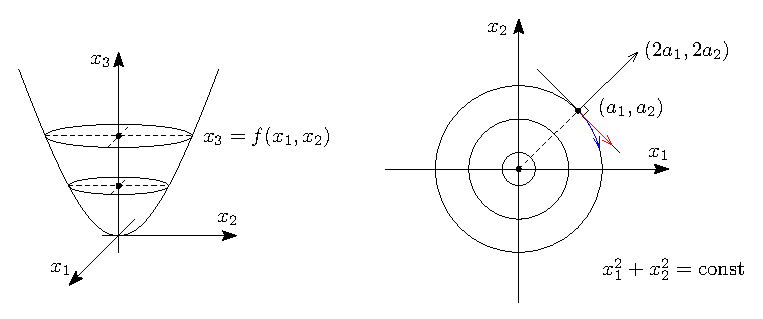
\includegraphics[width=0.8\textwidth]{12_2.eps}
	\caption{Поиск максимального возрастания функции $f$ с помощью линий уровня и градиента $(2a_1, 2a_2)$.}
	\label{12_2}
\end{figure}
Видно, что вектор градиента перпендикулярен линии уровня и это отражает наше наблюдение, что если двигаться перпендикулярно, то значения функции не должны изменяться. Как раз если будем сдвигаться перпендикулярно градиенту (красная линия), то будем двигаться вдоль линии уровня (синяя линия) и тем самым значение функции будет постоянным.

Если будем двигаться в сторону градиента, то функция будет максимально увеличиваться. Минус градиент будет направлен к нулю и если будем двигаться вдоль него, то функция будет максимально уменьшаться.

\begin{rem}
	На этой идее построен метод градиентного спуска.
\end{rem}

\end{document}